%! Author = adnansiddiquei
%! Date = 13/12/2023

\subsection{Q3 - Dataset C}\label{subsec:dataset-c}
    \begin{figure}
    \centering
    \begin{subfigure}{0.9\textwidth}
        \centering
        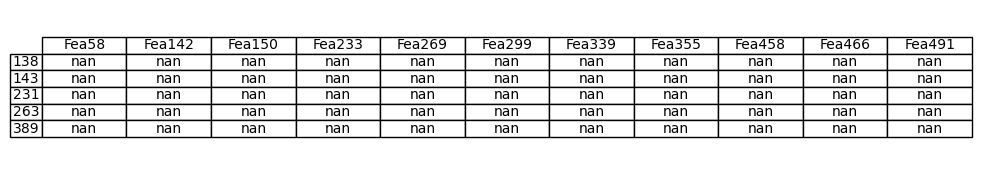
\includegraphics[width=1\textwidth]{./figures/q3a}
        \caption{The samples and features with missing data.}
        \label{fig:q3a}
    \end{subfigure}%
    \hfill
    \begin{subfigure}{0.9\textwidth}
        \centering
        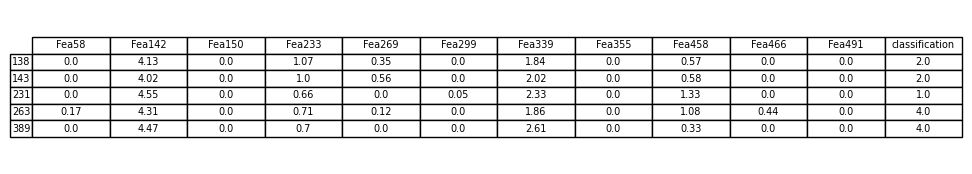
\includegraphics[width=1\textwidth]{./figures/q3c_1}
        \caption{The imputed data.}
        \label{fig:q3c}
    \end{subfigure}
    \caption{Samples and features with missing data, for the \inlinecode{C_MissingData.csv} dataset.}
    \label{fig:q3ac}
    \end{figure}

\subsubsection{Questions 3a and 3b}\label{subsubsec:q3ab}
    Fig\eqref{fig:q3a} shows all the features that have missing values, and all the samples which are missing
    those features.
    There are a few ways to handle missing data.
    A straightforward method is static imputation where every sample missing a given feature, is imputed with the same
    value for that feature, such as the mean of that feature.
    This is computationally inexpensive but can reduce the variance in the dataset and introduce bias if there are many
    missing values.
    Another method is model based imputation where an applicable model is chosen to estimate the value of the missing
    feature for each sample.
    An example is the K Nearest Neighbours approach, where a sample missing a feature is imputed with the mean of the
    K nearest neighbours.
    This can reduce the bias introduced and leave the variance unaffected, but highly dimensional data can often lead
    to less meaningful nearest neighbours, as distance can become less meaningful with more dimensions \cite{bellman1957}.

    Multiple imputation is where the missing data is imputed using a probabilistic model mutliple times, to create
    multiple datasets.
    The multiple imputed values can then either be averaged or the multiple datasets can then be individually analysed,
    Multiple imputation helps capture the uncertainty in what the missing data is, which is useful in the case that
    there is a large amount of missing data.

\subsubsection{Question 3c}\label{subsubsec:q3c}
    \begin{figure}[htb]
    \centering
    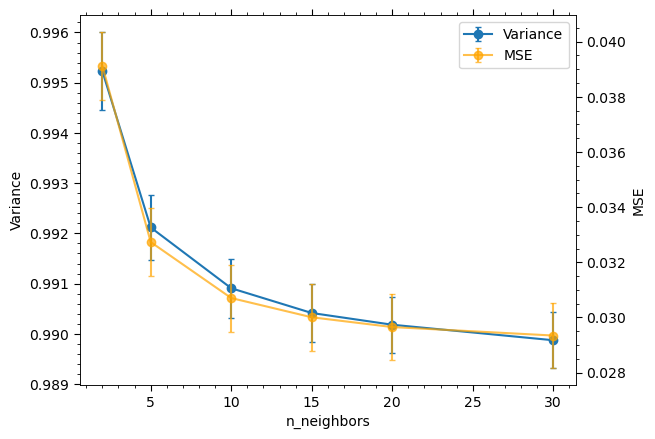
\includegraphics[width=0.9\textwidth]{./figures/q3c_optimise_knn_imputer}
    \caption{Variance and MSE of KNN imputed data, for different values of $k$. The variance is shown as a percentage
        of the original dataset, and the MSE is the mean squared error of predicted values against the true values.}
    \label{fig:q3c_optimise_knn_imputer}
    \end{figure}

    \begin{figure}[htb]
    \centering
    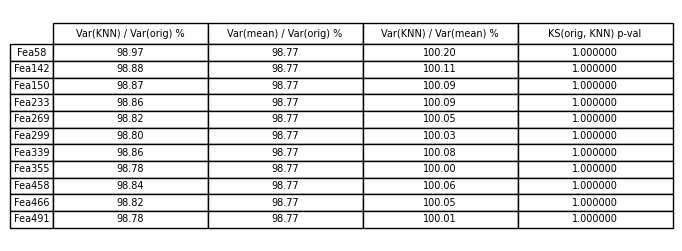
\includegraphics[width=0.9\textwidth]{./figures/q3c_2}
    \caption{A comparison of the variances of each feature after imputation. Column 1 shows the variance of each feature
        after KNN imputation, as a percentage of the original dataset. Column 2 shows this for mean imputation.
        Column 3 compares column 1 against column 2. Column 4 shows the p-value of the Kolmogorov-Smirnov test comparing
        the original dataset to the KNN imputed dataset.}
    \label{fig:q3c_2}
    \end{figure}

    Fig\eqref{fig:q3c_optimise_knn_imputer} was used to optimise the value of $k$ for the KNN imputation, and
    $k=15$ was chosen based on this simulation as further increase in $k$ did not significantly increase accuracy
    (a reduction in MSE).

    Fig\eqref{fig:q3c} shows the imputed data, with aforementioned KNN approach.
    However, PCA was performed first to reduce the dimensionality of the dataset, before the nearest neighbours were
    identified.
    Fig\eqref{fig:q3c_2} shows some summary and comparative statistics of the imputed data, which identifies that
    imputing the missing data did not significantly change the distributions of the features.

\subsubsection{Question 3d and 3e}\label{subsubsec:q3de}
    \begin{figure}[htb]
    \centering
    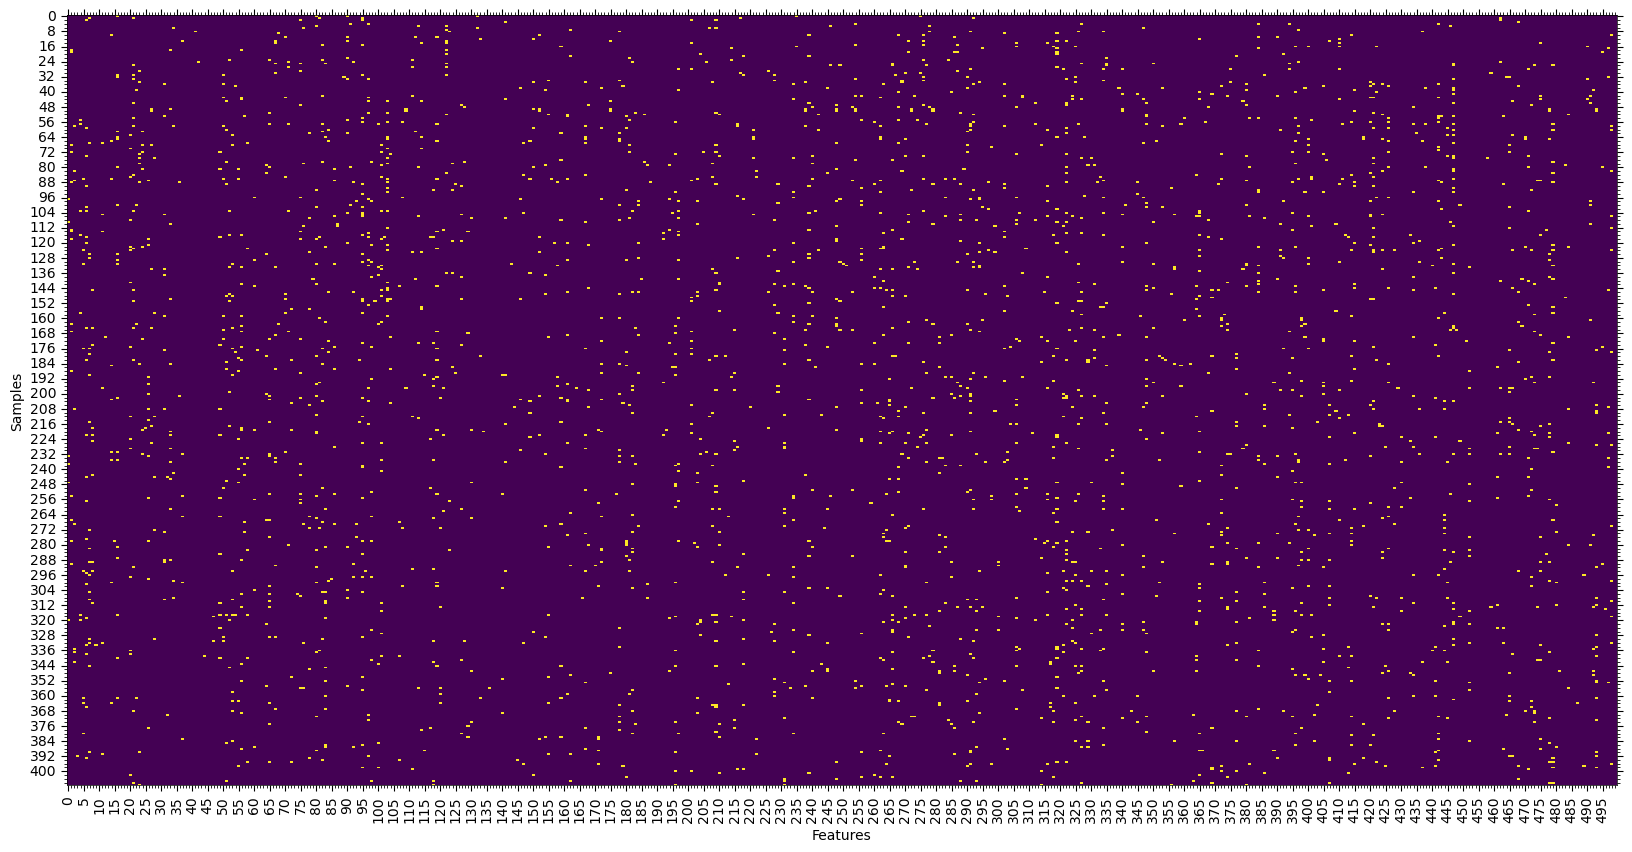
\includegraphics[width=1\textwidth]{./figures/q3d_heatmap}
    \caption{A heatmap of the outliers in the \inlinecode{C_MissingFeatures.csv} dataset. The orange marks indicate an
        outlier value, 2904 outlier values were identified.}
    \label{fig:q3d_heatmap}
    \end{figure}

    \begin{figure}[htb]
    \centering
    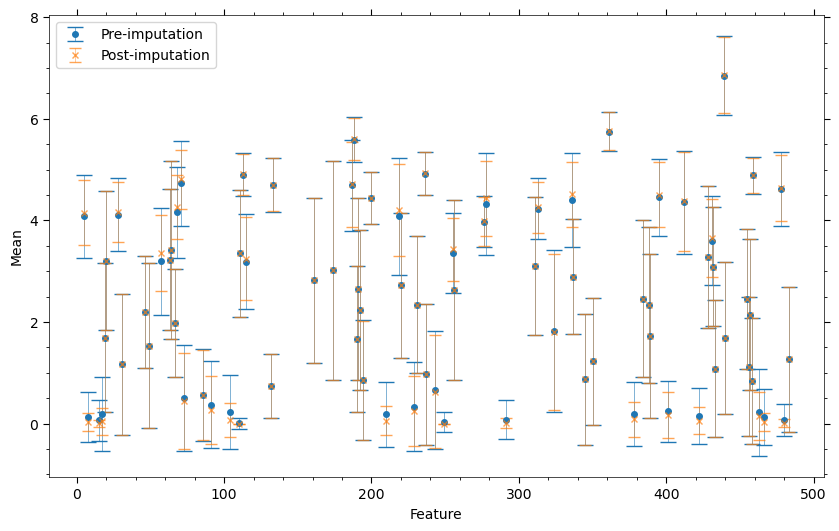
\includegraphics[width=0.9\textwidth]{./figures/q3e}
    \caption{The mean and standard deviation of the 81 most discriminative features in the original
        \inlinecode{C_MissingFeatures.csv} dataset, before and after outlier imputation.}
    \label{fig:q3e}
    \end{figure}

    Outlier values were identified by standardising the data feature-wise, and then identifying any values which were
    more than $3\sigma$ away from the mean.
    Fig\eqref{fig:q3d_heatmap} shows the outliers in the dataset, which shows that the outliers are fairly uniformly
    distributed across the dataset.

    These outliers were treated as missing values and imputed using the same dimensionality reduction and KNN imputation
    approach as utilised in Question 3c for missing values.
    The justification behind this is similar as that for Question 3c, the dataset is clustered and a distance based
    approach is therefore likely to be fruitful, and utilising dimensionality reduction allowed for identification of
    meaningful nearest neighbours.
    Outliers were removed iteratively, with the dataset being re-standardised and outliers being re-computed after each
    iteration.
    The algorithm iterated 8 times, until only 0.27\% of the data lay outside of $3\sigma$, which is the expected
    proportion of data outside of $3\sigma$ for a normal distribution.

    Fig\eqref{fig:q3e} shows the mean and standard deviation of the 81 most discriminative features (identified from
    the PCA loadings) before and after imputing the outliers.
    The variance of the features were reduced after imputation, which was expected, and the reduction in variance in the
    features with means close to zero was more significant as these features were more sparse and therefore more
    likely to have outliers.
